\documentclass[11pt]{article}

\usepackage[utf8]{inputenc}
\usepackage[T1]{fontenc}

\usepackage[a4paper, left=2cm, right=2cm, top=3.5cm, bottom=3.5cm]{geometry}
\usepackage[french]{babel}

% Paragraph spacing
\setlength{\parskip}{1em}

% Fancy headers
\usepackage{fancyhdr}

% Captions for subfigures
\usepackage{subcaption}

% Code highlighting
\usepackage{minted}

% Footnote inside a caption
\usepackage{fnpos}
\usepackage{ftnxtra}

% Maths
\usepackage{amsmath}
\usepackage{amssymb}

% Todo notes
\usepackage{todonotes}

% Table of contents for bibliography
\usepackage[nottoc]{tocbibind}

% Inline monospace font
\def\code#1{\texttt{#1}}

% Figures
\usepackage{graphicx}

% Draw figures
\usepackage{tikz}

% Tikz node rotation
\usetikzlibrary{positioning}

% Turing machine
\usetikzlibrary{chains,fit,shapes}

% Usage: \rotnode[options]{rotation}{text}
\newcommand\rotnode[3][]{%
    \node [#1, opacity=0.0] (tmp) {#3};
    \node [draw, rotate around={#2:(tmp.center)}] at (tmp) {#3};
}

% Clickable links
\usepackage{hyperref}

% Table of contents depth
\setcounter{tocdepth}{2}

% Inline code
\usepackage{listings}
\usepackage{color}

\title{Systèmes d'exploitation}

\author{William SCHMITT}
\date{2018-2019}

\begin{document}
\maketitle

\section{Introduction}
\subsection{Bibliographie}

Tanenbaum: Modern Operating Systems \\
Silberschatz: Operating Systems Concepts

\subsection{Plan}

\paragraph{Cours/TD}
\begin{itemize}
    \item Moniteurs
    \item Sémaphores
    \item futex
\end{itemize}

\paragraph{TP (pas à rendre)}
\begin{itemize}
    \item 1ère période : rappels de C
    \item 2ème période : mmap
\end{itemize}

\paragraph{TP (à rendre)}
\begin{itemize}
    \item Allocateur mémoire virtuel (malloc) : révisions sur les pointeurs
    \item Shell (fork, exec, redirection IO)
    \item Thread (lecteur vidéo multithread)
\end{itemize}

\paragraph{Présentation scientifique :} article de usenix.org (de 2019, 2018 ou dans les \textit{best papers} des 3 dernières années) à présenter devant la classe.

\subsection{Examen}
\begin{itemize}
    \item QCM: 1h (20 à 25 questions) \\
    \item TP: 
    \begin{itemize}
        \item 2h (75\%)
        \item Présentation scientifique (25\%)
    \end{itemize}
\end{itemize}


Notation : 50/50.

\subsection{Fibonacci}
Comparaison avec/sans printf, ratio de performance : 397

Avec redirection de stdout dans /dev/null, le ratio plonge à 31.

Lorsque les tampons sont pleins (dans le terminal), on bloque les producteurs de données le temps de vider les tampons (et donc d'afficher les résultats).

Facteurs décorrélés de l'algorithme permettant des gains :
\begin{itemize}
    \item IO
    \item Gestion de la mémoire
\end{itemize}

\section{Hardware}
On se base sur un modèle simpliste.
\begin{figure}
    \centering
    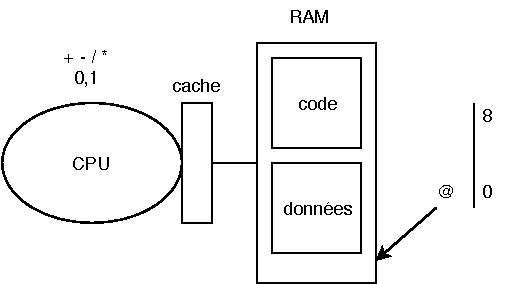
\includegraphics{img/cpu+ram.pdf}
\end{figure}

Depuis les années 1990, la vitesse du CPU a dépassé celle de la mémoire. En un cycle CPU (pour un CPU à 4GHz), un photon peut parcourir 7,5cm. On rajoute à cette époque du cache dans les CPU pour compenser la lenteur de la mémoire.

De plus, la taille de la mémoire a explosé.

\section{Système d'exploitation}
Dans les premier ordinateurs, on réglait l'état mémoire à la main avec des interrupteurs.

\begin{figure}
    \centering
    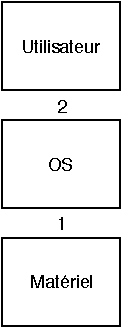
\includegraphics{img/hw-os-user.pdf}
\end{figure}

Un OS est à la base composé de différentes routines qui ont deux buts :
\begin{enumerate}
    \item Gestion du matériel (partage, arbitrage, partition, droits/utilisateurs) \begin{itemize}
        \item Processeurs (dont la complexité augmente)
        \item Disques/SSD/Burst buffer/Bandes magnétiques
        \item RAM
        \item Interfaces réseau
    \end{itemize}
    \item Abstractions
    \begin{itemize}
        \item Fichiers, répertoires, systèmes de fichiers
        \item processus
        \item utilisateurs
        \item socket réseau
    \end{itemize}
\end{enumerate}

\subsection{Composition d'un OS}
Le noyau Linux est constitué d'environ 18 millions de lignes en C. Ingérable par une seule personne, il est décomposé en modules exposant des API puis compilé en un programme comme les autres, à quelques exceptions près.

\paragraph{Mode d'exécution} un OS s'exécute dans un mode spécial et a accès à des instructions spéciales. 

\paragraph{Interruptions et exceptions} permettent de passer du mode user au mode kernel. La différence entre les deux : les interruptions sont masquables.

\paragraph{Bibliothèque système côté utilisateur} permettant (notamment) d'éviter de coder les interruptions à la main.

S'il s'agit d'un programme comme les autres : où et quand est-il en RAM ? Où et quand s'exécute-t-il ?

Il est toujours en RAM (notamment pour pouvoir répondre aux interruptions), avec certaines nuances : tout l'OS n'est pas en mémoire ! Pour Linux, seuls certains modules sont chargés, notamment pour des drivers. Sous Windows, les parties non utilisées sont sur disque (swap).

En termes d'exécution, il n'est exécuté que lors d'interruptions/exceptions.

Déroulement du boot
\begin{itemize}
    \item Intel ME (management engine), codé sur le processeur et peut faire tourner Minix.
    \item BIOS/UEFI : exécuté directement par le CPU au boot, accessible comme de la mémoire normale, pour chercher le chargeur et le mettre en mémoire. Fourni par le fabricant de mobo, il y a déjà des interactions avec le matériel avant le chargement de l'OS. L'accroissement de complexité de l'UEFI (possibilité de surfer) présente des problématiques de sécurité.
    \item Chargeur : mise en RAM des données sur disque \begin{itemize}
        \item Windows
        \item GRUB
        \item Autre...
    \end{itemize}
    \item Initialisation
    \item Vecteurs d'interruption/exception
\end{itemize}

La maîtrise de la machine physique devient de plus en plus lointaine, même au niveau des OS.

\subsection{Modularité}
\begin{figure}[ht]
    \centering
    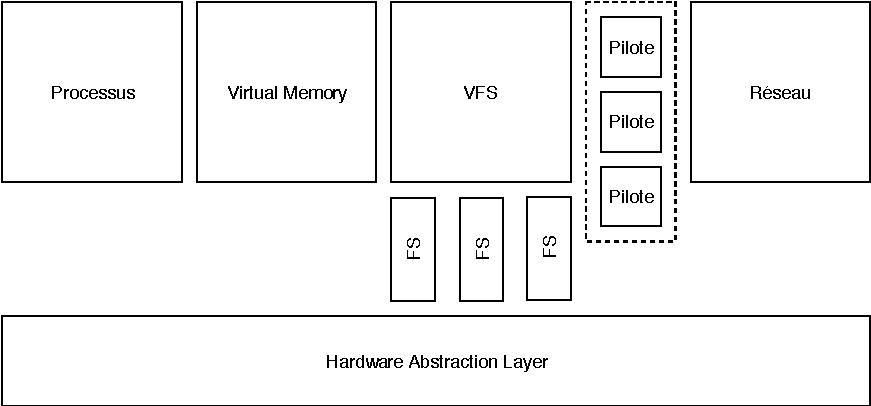
\includegraphics{img/modular-os.pdf}
\end{figure}

Les \textbf{systèmes de fichier virtuels} sont une API haut niveau pour l'ouverture, la fermeture, la lecture, l'écriture de fichiers. Les filesystems sont par exemple ext4, btrfs, fat, fat32, ntfs.

\subsection{Histoire}
"L'histoire de l'informatique, ça remonte aux machines automatiques pour faire des trucs."
\subsubsection{Préhistoire}
\begin{itemize}
    \item Babylone
    \item Machine Héron d'Alexandrie
\end{itemize}

\subsubsection{Histoire}
\paragraph{Epoque mécanique}
\begin{itemize}
    \item Pascal
    \item Babbage: machine universelle programmable
    \item Ada Lovelace (if, boucle)
\end{itemize}

\paragraph{Antiquité}
\begin{itemize}
    \item Turing
    \item ENIAC
\end{itemize}

\paragraph{Moyen-Âge}
\begin{itemize}
    \item IO: cartes perforées
    \item Tampon: copie des IO en RAM
\end{itemize}

\paragraph{Monde moderne (1960)}
\begin{itemize}
    \item MULTICS: OS moderned (processus, droits, fichiers, multi-utilisateurs)
    \item 1969 : Mini-ordinateur: PDP11
    \item UNIX : (asm pour la première version, C pour la deuxième)
    \item 1974 : Micro-ordinateurs
    \begin{itemize}
        \item Grand public : pas assez puissants pour faire tourner UNIX, donc utilisation de CP/M (8 bits, 16ko RAM) puis DOS en 1981
        \item Station de travail : permettent de faire tourner UNIX
    \end{itemize}
    \item 1987 : Minix, reste petit pour permettre d'être un outil pédagogique (bouquin avec src + explication)
    \item 1991 : Linux \begin{itemize}
        \item internet
        \item GPL : possibilité de voir et modifier le code, obligation de distribuer le code modifié
    \end{itemize}

\end{itemize}

\end{document}